\documentclass{article}
\usepackage{hyperref}
\usepackage{Style}

\nocite{*} % Comentar si quiero citar
%\addbibresource{bibliografia.bib} % Quitar el comentado si quiero usar bibliografia

\begin{document}

\begin{minipage}{2.5cm}
    \includegraphics[width=2cm]{imagen_puc.jpg}
\end{minipage}
\begin{minipage}{14cm}
    {\sc Pontificia Universidad Católica de Chile\\
    Facultad de Matemáticas\\
    Departamento de Matemática\\
    Profesor: Mauricio Bustamante -- Estudiante: Benjamín Mateluna}
\end{minipage}
\vspace{1ex}

{\centerline{\bf Topología Algebraica - MAT2850}
\centerline{\bf Apuntes}}
\centerline{\bf 05 de agosto de 2025}

\newpage
\tableofcontents

\newpage
\section*{Motivación}
\phantomsection
\addcontentsline{toc}{section}{Motivación}
\noindent Dados dos espacios topológicos $X$ e $Y$ ¿Cuando son homeomorfos?. Decimos que dos 
espacios son \textbf{homeomorfos} si existe $f:X\to Y$ continua, biyectiva y con inversa 
constinua. La topología algebraica ataca esta pregunta de la siguiente forma:
\begin{enumerate}
    \item Asigna a cada espacio topológico $X$ un objeto algebraico $G(X)$.
    \item Aigna a cada función continua $f:X\to Y$ un homomorfismo $G(f):G(X)\to G(Y)$ tal que
    \begin{enumerate}
        \item $G(f\circ g)=G(f)\circ G(g)$
        \item $G(id_{X})=id_{G(X)}$
    \end{enumerate}
\end{enumerate}
\noindent\textbf{Observación:} Ambas condiciones implican que si $f:X\to Y$ es homeomorfismo, 
entonces $G(f):G(X)\to G(Y)$ es isomorfismo. A veces los $G$ que se construyen satisfacen la 
propiedad extra que si $X$ se puede ''deformar continuamente'' en $Y$ entonces $G(X)\cong G(Y)$.

\vspace{2mm}
\noindent Decimos que $G$ es un \textbf{invariante homotópico}.

\noindent\textbf{Ejemplos:}
\begin{enumerate}
    \item Tenemos los espacios
    \begin{center} %Ilustraciones de la esfera y el toro
        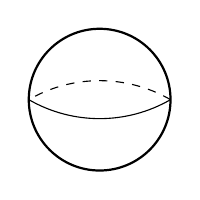
\begin{tikzpicture}[scale=0.9]
            \coordinate (A) at (0,0,0);
            \coordinate (B) at (-1,0,0);
            \coordinate (C) at (1,0,0);

            \filldraw[color=black, fill=white, thick] (A) circle (1);
            \draw (B) arc (240:300:2);
            \draw[dashed] (C) arc (60:120:2);
        \end{tikzpicture}
        %
        \hspace{2cm}
        %
        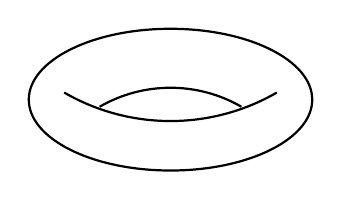
\begin{tikzpicture}[scale=0.9]
            \coordinate (A) at (0,0);
            \coordinate (B) at (-1.5,0.1);
            \coordinate (C) at (1,-0.1);

            \draw[thick] (A) ellipse (2cm and 1cm);
            \draw[thick] (B) arc (240:300:3);
            \draw[thick] (C) arc (60:120:2);
        \end{tikzpicture}
    \end{center}
    Mas adelante veremos que la homología le asigna a la esfera el grupo $\{e\}$ y al toro 
    $\Z^{2}$. En general, una superficie de genero $g$ tendrá el grupo $\Z^{2g}$.

    \item ¿Cuando $\R^{n}$ y $\R^{m}$ son homeomorfos? Si $n\neq$, el grupo de homología de 
    $\R^{n}$ será $\{e\}$ y por el contrario, para $\R^{m}$ va a ser $\Z$ y por lo tanto $R^{n}$ y
    $\R^{m}$ son homeomorfos si y solo si $n=m$.

    \item Un ejemplo particular, para el circulo se tiene que $\pi_{1}(\s^{1})=\Z$ pero 
    $\pi_{1}(\s^{2})=\{e\}$ y por lo tanto los espacios no son homeomorfos.
\end{enumerate}

\vspace{2mm}
\begin{dfn}
    Una \textbf{homotopía} entre dos funciones continuas $f,g:X\to Y$ es una función continua 
    $H:X\times[0,1]\to Y$ tal que $H(x,0)=f(x)$ y $H(x,1)=g(x)$ para todo $x\in X$.
\end{dfn}
\noindent\textbf{Notación:} La función $H_{t}:X\to Y$ esta dada por $H_{t}(x):=H(x,t)$. Una 
homotopía de $f$ a $g$ se denota por $f\sim g$.

\vspace{2mm}
\begin{prop}
    Ser homotópico es una relación de equivalencia en $\mathcal{C}(X,Y)$.
\end{prop}
\begin{proof}
    Debemos probar tres cosas
    \begin{enumerate}
        \item La relación es reflexiva. Sea $f:X\to Y$, consideramos la homotopía constante, esto
        es $H(x,t):=f(x)$ es continua ya que

        \centerline{
            \xymatrix{
                X\times[0,1] \ar[r]^-{\pi_{X}} \ar@/_0.8pc/[rr]_{H} & X \ar[r]^-{f} & Y
            }
        }
        \item Simetría. Supongamos que $f\sim g$, consideramos $H'(x,t)=H(x,1-t)$ y es continua
        por que
        
        \vspace{2mm}
        \centerline{
            \xymatrixcolsep{3pc}\xymatrix{
                X\times[0,1] \ar[r]^-{id\times(1-t)} \ar@/_1.1pc/[rr]_{H'} & X\times[0,1]
                \ar[r]^-{H} & Y
            }
        }
        \item Por último, la transitividad. Sean $f\sim g$ y $g\sim h$, Definimos 
        $H*G:X\times[0,1]\to Y$ dada por
        \begin{equation*}
            H*G(x,t):=\begin{cases}
                H(x,2t) &\quad\text{ si}\hspace{2mm}0\leq t\leq\frac{1}{2} \\
                G(x,2t-1) &\quad\text{ si}\hspace{2mm}\frac{1}{2}\leq t\leq1
            \end{cases}
        \end{equation*}
        que resulta continua por el lema del pegado.
    \end{enumerate}
\end{proof}

\newpage
\vspace{2mm}
\begin{dfn}
    Decimos que $f:X\to Y$ es una \textbf{equivalencia homotópica}, si existe $g:Y\to X$ tal que 
    $g\circ f\sim id_{X}$ y $f\circ g\sim id_{Y}$
\end{dfn}
\noindent En tal caso, $X$ e $Y$ se dicen homotópicamente equivalentes o que tienen el mismo tipo 
de homotopía y se denota por $X\sim Y$.

\vspace{2mm}
\noindent\textbf{Ejemplo:}
\begin{enumerate}
    \item Sea $f:X\to Y$ un homeomorfismo, en particular, tomando $g=f^{-1}$, se sigue que es 
    equivalencia homotópica.

    \item Se tiene que $\{0\}\sim\R^{n}$, consideremos la inclusión $i:\to\{0\}\to\R^{n}$, 
    afirmamos que es $i$ es equivalencia homotópica. En efecto, se verifica que $\pi:\R^{n}\to
    \{0\}$ es una inversa homotópica. Por un lado $\pi\circ i=id_{\{0\}}$ y por otro 
    $i\circ\pi=0$. Notamos que $H(x,t)=tx$ con $t\in[0,1]$ es una homotopía entre $0$ y 
    $id_{\R^{n}}$.

    \item Veamos que $\R^{n}\setminus\{0\}\sim\s^{n-1}$. Probaremos que la función 
    $i:\s^{n-1}\to\R^{n}\setminus\{0\}$ es equivalencia homotópica. En efecto,
    \begin{align*}
        \pi:\R^{n}\setminus\{0\} &\to \s^{n-1} \\
        x &\to \frac{x}{\abs{x}}
    \end{align*}
    es inversa homotópica. Es claro que $\pi\circ i=id_{s^{n-1}}$. Definimos
    \begin{equation*}
        H(x,t):=t\frac{x}{\abs{x}}+(1-t)x
    \end{equation*}
    Notamos que $H(x,0)=x$ y $H(x,1)=\frac{x}{\abs{x}}$, es decir, $H$ es una homotopia entre 
    $i\circ\pi$ e $id_{\R^{n}\setminus\{0\}}$. Además, se verifica que 
    $im(H)\subseteq\R^{n}\setminus\{0\}$.
\end{enumerate}

\newpage
\section{Homología Simplicial}
\noindent Queremos asignarle a un espacio topológico $X$ arbitrario, grupos abelianos 
$H_{0}(X),H_{1}(X),\cdots$ tal que si $X\sim Y$, entonces $H_{i}(X)\cong H_{i}(Y)$ para todo $i$.
Ituitivamente, $H_{k}(X)$ estará generado por ciertos subespacios de $X$ de dimensión $k$.

\vspace{2mm}
\noindent Habrá una relación de equvalencia, $A,B\subseteq X$ de dimensión $k$ serán equivalentes
si hay un subespacio de $X$ de dimensión $k+1$ cuyo borde es $A\cup B$.

\vspace{2mm}
\noindent Hay que restringir la clase de espacios a una con nociones de dimensión, borde, etc. 
Estos serán los complejos simpliciales. Necesitamos, adicionalmente, un objeto algebraico que 
capture esas nociones, esto corresponde a los complejos de cadenas.

\subsection{Complejos de Cadenas}
\begin{dfn}
    Un \textbf{complejo de cadenas} es una sucesión de grupos abelianos y homomorfismos
    
    \vspace{2mm}
    \centerline{
        \xymatrix{
            \cdots \ar[r] & C_{3} \ar[r]^{\partial_{3}} & C_{2} \ar[r]^{\partial_{2}} & 
            C_{1} \ar[r]^{\partial_{1}} & C_{0} \ar[r] & 0
        }
    }
    \vspace{2mm}
    \noindent tal que $d_{i}\circ d_{i+1}=0$ para todo $i$. Se denota por $(C_{*},d_{*})$.
\end{dfn}
\noindent\textbf{Observación:} Notemos que $\im{d_{i+1}}\subseteq\kr{d_{i}}\subseteq C_{i}$. Dado 
que los grupos son abelianos, esta observación permite definir el siguiente objeto.

\vspace{2mm}
\begin{dfn}
    El \textbf{i-ésimo grupo de homología} de $(C_{*},d_{*})$ se define por
    \begin{equation*}
        H_{i}(C_{i}):=\frac{\kr{d_{i}}}{\im{d_{i+1}}}
    \end{equation*}
\end{dfn}

\vspace{2mm}
\noindent\textbf{Ejemplos:}
\begin{itemize}
    \item Si $A$ un grupo abeliano, entonces
    
    \vspace{2mm}
    \centerline{
        \xymatrix{
            \cdots \ar[r] & 0 \ar[r] & 0 \ar[r] & A \ar[r] & 0 \ar[r] & \cdots \ar[r] & 0
        }
    }
    \vspace{2mm}
    es un complejo de cadenas donde $C_{i}=A$. Entonces
    \begin{equation*}
        H_{j}(C_{*})=\begin{cases}
            0 & \quad\text{si }j\neq i \\
            A & \quad\text{si }j=i
        \end{cases}
    \end{equation*}

    \item Consideremos la cadena exacta
    
    \vspace{2mm}
    \centerline{
        \xymatrix{
            \cdots \ar[r] & 0 \ar[r] & \Z \ar[r]^{\cdot2} & \Z \ar[r]^{\pi} & \Z_{2} \ar[r] & 0
        }
    }
    \vspace{2mm}
    entonces $H_{j}(C_{*})=0$ para todo $i$.

    \item Veamos que
    
    \vspace{2mm}
    \centerline{
        \xymatrix{
            \cdots \ar[r] & \Z \ar[r]^{\cdot2} & \Z \ar[r]^{\cdot0} & \Z \ar[r] & 0
        }
    }
    \vspace{2mm}    
    es un complejo de cadenas. La homología asociadas son $H_{0}(C_{*})=\Z$, $H_{1}(C_{*})=\Z_{2}$
    y $H_{k}(C_{*})=0$.
\end{itemize}

\begin{dfn}
    Sean $(C_{*},\partial_{*})$ y $(D_{*},\partial_{*})$ dos complejos de cadenas. Un 
    \textbf{mapeo de cadenas} es una colección de homomorfismos $f_{n}:C_{n}\to D_{n}$ tal que 
    $\partial_{n}f_{n}=f_{n-1}\partial_{n}$ para todo $n$, es decir, el siguiente diagrama conmuta

    \vspace{2mm}
    \centerline{
        \xymatrix{
            C_{n} \ar[r]^{\partial_{n}} \ar[d]^{f_{n}} & C_{n-1} \ar[d]^{f_{n-1}} \\
            D_{n} \ar[r]^{\partial_{n}} & D_{n-1}
        }
    }
    \noindent y se denota por $(f):C_{*}\to D_{*}$.
\end{dfn}

\vspace{2mm}
\begin{lema}
    Si $(f):C_{*}\to D_{*}$ es un mapeo de cadenas, entonces la asignación 
    $f_{*}:H_{n}(C_{*})\to H_{n}(D_{*})$ dada por
    \begin{equation*}
        f_{*}([x])=[f_{n}(x)]
    \end{equation*}
    esta bien definida y es un homomorfismo de grupos.
\end{lema}
\begin{proof}
    Sea $x\in ker\partial_{n}$ entonces $\partial_{n}f_{n}(x)=f_{n-1}\partial_{n}(x)
    =f_{n-1}(0)=0$. Así, $f_{n}(x)\in\kr{\partial_{n}}$ y por tanto la expresión tiene sentido. Si
    $[x]=[y]$ entonces $x-y=\partial_{n}(z)$ para $z\in C_{n+1}$, se sigue que 
    $f_{n}(x)-f_{n}(y)=f_{n}\partial_{n+1}(z)=\partial_{n+1}f_{n+1}(z)$. Concluimos que 
    $[f_{n}(x)]=[f_{n}(y)]$.
\end{proof}

\noindent\textbf{Ejemplo:}
Consideremos la siguiente situación

\vspace{2mm}
\centerline{
    \xymatrix{
        \cdots \ar[r] & 0 \ar[r]^{0} \ar[d] & \Z \ar[r]^{3} \ar[d]^{id} & 
        \Z \ar[r]^{0} \ar[d]^{\pi} & \Z \ar[r] \ar[d]^{id} & 0 & C_{*} \ar[d]^{(f)} \\
        \cdots \ar[r] & 0 \ar[r]^{0} & \Z \ar[r]^{3} & \Z_{3} \ar[r]^{0} & \Z \ar[r] & 0 & D_{*}
    }
}
\vspace{2mm}
\noindent Entonces $f_{*}:H_{2}(C_{*})=0\to H_{2}(D_{*})=\Z$ es el morfismo trivial. Mientras que
$\pi_{*}:H_{1}(C_{*})=\Z_{3}\to H_{1}(D_{*})=\Z_{3}$ es la identidad.

\vspace{2mm}
\noindent\textbf{Observación:} Sea $(g):D_{*}\to G_{*}$ un mapeo de cadenas, entonces 
$(g\circ f):C_{*}\to G_{*}$ es un mapeo de cadenas y el siguiente diagrama conmuta

\vspace{2mm}
\centerline{
    \xymatrix{
        H_{n}(C_{*}) \ar[rr]^{(g\circ f)_{*}} \ar[rd]^{f_{*}} & & H_{n}(G_{*}) \\
         & H_{n}(D_{*}) \ar[ru]^{g_{*}}
    }
}
\vspace{2mm}
\noindent Notemos que $\partial_{n}g_{n} f_{n}=g_{n-1}\partial_{n}f_{n}=g_{n-1}f_{n-1}
\partial_{n}$. Por otro lado, tenemos que $(g\circ f)_{*}([x])=[(g\circ f)(x)]=g_{*}([f(x)])=
(g_{*}\circ f_{*})([x])$, lo que prueba la afirmación.

\vspace{2mm}
\noindent Nuestro objetivo será asociar un complejo de cadenas a un espacio topológico $X$ 
arbitrario, lo que nos dara un grupo de homología para cada dimensión, además dada $f:X\to Y$ una
función continua, nos gustaría obtener un mapeo de cadenas y por tanto un homomorfismo entre los
grupos de homología de cada espacio.

\newpage
\subsection{Complejos Simpliciales}
\begin{dfn}
    Dados $n+1$ puntos $\{v_{0},\cdots,v_{n}\}\in\R^{\omega}$ son \textbf{afínmente 
    independientes}, si generan un $n-$plano afín, es decir, $\{v_{1}-v_{0},\cdots,v_{n}-v_{0}\}$
    es un conjunto linealmente independiente, esto es
    \begin{equation*}
        \sum_{i=0}^{n}t_{i}v_{i}=0\hhtext{y}\sum_{i=0}^{n}t_{i}=0
        \hhtext{entonces}t_{i}=0\text{ para todo }i
    \end{equation*}
\end{dfn}

\vspace{2mm}
\noindent\textbf{Ejemplo:} Dos puntos son afínmente independientes. Tres puntos son afínmente 
independientes si y solo si no son colineales.

\vspace{2mm}
\begin{dfn}
    Si $\{v_{0},\cdots,v_{n}\}$ son afínmente independientes, ellos definen el \textbf{n-simplejo}
    \begin{equation*}
        \sigma=\gen{v_{0},\cdots,v_{n}}=\left\{x=\sum_{i=0}^{n}t_{i}v_{i},\hspace{2mm}
        \sum_{i=0}^{n}t_{i}=1\hhtext{y}t_{i}\geq0\right\}
    \end{equation*}
\end{dfn}

\noindent Decimos que $\sigma$ es el $n-$simplejo generado por $v_{0},\cdots,v_{n}$. Los puntos 
$v_{i}$ se llaman \textbf{vértices} de $\sigma$. Una \textbf{cara} de un simplejo $\sigma$ es 
un simplejo $\tau$ generado por un subconjunto de $\{v_{0},\cdots,v_{n}\}$ y lo denotamos por 
$\tau\leq\sigma$. Si el subconjunto es propio, se dice que $\tau$ es una \textbf{cara propia}.

\vspace{2mm}
\noindent La \textbf{frontera} de un $n-$simplejo $\sigma$ es la unión de todas sus caras propias, 
se denota por $\partial\sigma$, el \textbf{interior} de $\sigma$ es $int(\sigma):=
\sigma\setminus\partial\sigma$.

\begin{center}
    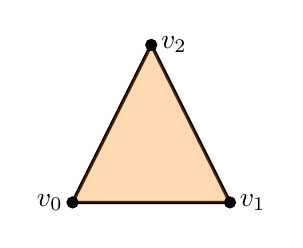
\begin{tikzpicture} %Un 2-simplejo
        \coordinate (A) at (0,0);
        \coordinate (B) at (2,0);
        \coordinate (C) at (1,2);

        \draw[very thick] (A) -- (B) -- (C) -- cycle;
        \fill[color=orange, opacity=0.3] (A) -- (B) -- (C) -- cycle;

        \filldraw (C) circle (2pt) node[anchor=west]{$v_{2}$};
        \filldraw (B) circle (2pt) node[anchor=west]{$v_{1}$};
        \filldraw (A) circle (2pt) node[anchor=east]{$v_{0}$};
    \end{tikzpicture}
\end{center}

\vspace{2mm}
\begin{dfn}
    Un \textbf{complejo simplicial} (geométrico) $K$ es un conjunto de simplejos tales que
    \begin{enumerate}
        \item Si $\sigma\in K$ y $\tau\leq\sigma$ entonces $\tau\in K$.
        \item Si $\sigma,\tau\in K$ entonces $\sigma\cap\tau=\emptyset$ ó $\sigma\cap\tau$ es una
        cara de $\sigma$ y de $\tau$.
    \end{enumerate}
\end{dfn}
\noindent El \textbf{poliedro} asociado a un complejo simplicial $K$ es 
$\abs{K}:=\bigcup_{\sigma\in K}\sigma$. Un espacio topológico $X$ se llama un poliedro si existe
un complejo simplicial $K$ y un homeomorfismo $f:\abs{K}\to X$. Al par $(K,f)$ se le llama una 
\textbf{triangulación} de $X$. Denotamos por $V_{K}$ al conjunto de vértices de los simplices.

\vspace{2mm}
\noindent\textbf{Observación:} Si $X$ es triangulable, entonces es Hausdorff por que $\abs{K}$ 
lo es.

\begin{center}
    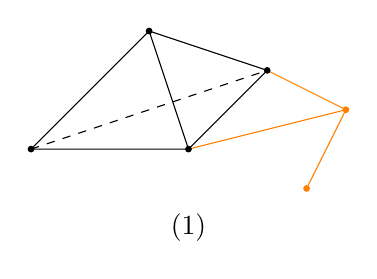
\begin{tikzpicture} %Ejemplo de complejo simplicial
        \coordinate (A) at (0,0);
        \coordinate (B) at (2,0);
        \coordinate (C) at (3,1);
        \coordinate (D) at (1.5,1.5);
        \coordinate (E) at (4,0.5);
        \coordinate (F) at (3.5,-0.5);

        \draw (A) -- (B) -- (D) -- cycle;
        \draw (D) -- (C) -- (B);
        \draw[dashed] (A) -- (C);
        \draw[color=orange] (B) -- (E) -- (C);
        \draw[color=orange] (E) -- (F);

        \filldraw (A) circle (1pt);
        \filldraw (B) circle (1pt);
        \filldraw (C) circle (1pt);
        \filldraw (D) circle (1pt);
        \filldraw[color=orange] (E) circle (1pt);
        \filldraw[color=orange] (F) circle (1pt);

        \node at (2,-1) {(1)};
    \end{tikzpicture}
    %
    \hspace{2cm}
    %
    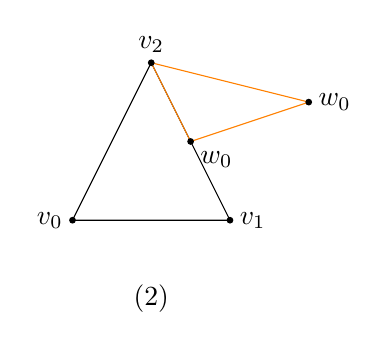
\begin{tikzpicture} %Ejemplo de un no complejo simplicial
        \coordinate (A) at (0,0);
        \coordinate (B) at (2,0);
        \coordinate (C) at (1,2);
        \coordinate (D) at (1.5,1);
        \coordinate (E) at (3,1.5);

        \draw (A) -- (B) -- (C) -- cycle;
        \draw[color=orange] (C) -- (D) -- (E) -- cycle;

        \filldraw (A) circle (1pt) node[anchor=east]{$v_{0}$};
        \filldraw (B) circle (1pt) node[anchor=west]{$v_{1}$};
        \filldraw (C) circle (1pt) node[anchor=south]{$v_{2}$};
        \filldraw (D) circle (1pt) node[anchor=north west]{$w_{0}$};
        \filldraw (E) circle (1pt) node[anchor=west]{$w_{0}$};

        \node at (1,-1) {(2)};
    \end{tikzpicture}
\end{center}
\noindent La figura $(1)$ corresponde a un complejo simplicial, mientras que la figura $(2)$ no
es un complejo simplicial ya que los simplices que la componen no se pegan bien.

\vspace{2mm}
\noindent\textbf{Ejemplo:} Consideremos el complejo simplicial $K$ formado por los simplices 
$\sigma=\gen{\pm e_{1},\pm e_{2}, \pm e_{3}}$ y sus respectivas caras. Consideremos 
$f:\abs{K}\to\s^{2}$ por $f(x):=x/\abs{x}$, entonces $(K,f)$ es una triangulación de la 
$2-$esfera.

\begin{center}
    \begin{tikzpicture}[scale=0.9] %Representación del complejo simplicial
        \coordinate (O) at (0,0);
        \coordinate (A) at (-0.5,-1);
        \coordinate (B) at (1,0);
        \coordinate (C) at (0,1);

        \draw (O) -- ($1.5*(A)$);
        \draw (O) -- ($1.5*(B)$);
        \draw (O) -- ($1.5*(C)$);

        \draw[dashed] (O) -- ($-1.5*(A)$);
        \draw[dashed] (O) -- ($-1.5*(B)$);
        \draw[dashed] (O) -- ($-1.5*(C)$);

        \draw[orange] (A) -- (B) -- (C) -- cycle;
        \draw[orange] (A) -- (B) -- ($-1*(C)$) -- cycle;
        \draw[orange] (A) -- ($-1*(B)$) -- (C) -- cycle;
        \draw[orange] ($-1*(A)$) -- (B) -- (C) -- cycle;

        \draw[orange, dashed] ($-1*(B)$) -- ($-1*(C)$);
        \draw[orange, dashed] ($-1*(B)$) -- ($-1*(A)$);
        \draw[orange, dashed] ($-1*(A)$) -- ($-1*(C)$);

        \filldraw (A) circle (1pt) node[anchor=north west]{$e_{1}$};
        \filldraw (B) circle (1pt) node[anchor=north west]{$e_{2}$};
        \filldraw (C) circle (1pt) node[anchor=south west]{$e_{3}$};
    \end{tikzpicture}
\end{center}

\vspace{2mm}
\begin{dfn}
    Sean $K$ y $L$ complejos simpliciales. Un \textbf{mapeo simplicial} de $K$ a $L$ es una 
    función $f:V_{K}\to V_{L}$ tal que si $\sigma=\gen{v_{\alpha_{0}},\cdots,v_{\alpha_{n}}}$ es
    un simplejo en $K$ entonces
    \begin{equation*}
        \{f(v_{\alpha_{0}}),\cdots,f(v_{\alpha_{n}})\}
    \end{equation*}
    genera un simplice en $L$, al cual llamamos $f(\sigma)$. Notación $f:K\to L$.
\end{dfn}

\vspace{2mm}
\noindent\textbf{Ejemplo:} Sea $\triangle^{n}=\gen{e_{1},\cdots,e_{n+1}}\subseteq\R^{n+1}
\subseteq\R^{\infty}$. Entonces las funciones $f:\triangle^{1}\to\triangle^{2}$ y 
$g:\triangle^{2}\to\triangle^{1}$ dadas por $f(e_{i})=e_{i}$ y $g(e_{1})=g(e_{3})=e_{1}$, 
$g(e_{2})=e_{2}$ son mapeos simpliciales.

\vspace{2mm}
\begin{lema}
    Sea $f:K\to L$ un mapeo simplicial. Entonces induce una función continua 
    $\abs{f}:\abs{K}\to\abs{L}$.
\end{lema}
\begin{proof}
    Sea $\sigma\in K$, digamos que $\sigma=\gen{v_{\alpha_{0}},\cdots,v_{\alpha_{n}}}$ y Definimos
    \begin{align*}
        f_{\sigma}:\sigma &\to \abs{L} \\
        \sum_{i=0}^{k}t_{i}v_{i} &\to \sum_{i=0}^{k}t_{i}f(v_{i})
    \end{align*}
    que es continua por que es lineal en los $t_{i}$. Se observa que si $\tau\leq\sigma$ entonces
    $f_{\tau}=f_{\sigma}\big|_{\tau}$. Ahora tomamos $\sigma$ y $\sigma'$, entonces
    \begin{equation*}
        f_{\sigma}\big|_{\sigma\cap\sigma'}=f_{\sigma\cap\sigma'}
        =f_{\sigma'}\big|_{\sigma\cap\sigma'}
    \end{equation*}
    entonces $\abs{f}:=\bigcup_{\sigma\in K}f_{\sigma}$ es una función continua de $\abs{K}$ en 
    $\abs{L}$.
\end{proof}
\noindent Se verifica también que $\abs{g\circ f}=\abs{g}\circ\abs{f}$. Un mapeo simplicial puede
ser definido también como una función continua $f:\abs{K}\to\abs{L}$ que manda vértices en
vértices y es lineal en sus caras.

\newpage
\subsection{Homología Simplicial}
\noindent Dado $K$ un complejo simplicial finito, esto es, que tiene un número finito de vértices. 
Elegimos un orden total en el conjunto de vértices, digamos $v_{0}<v_{1}<\cdots<v_{n}$.

\vspace{2mm}
\begin{dfn}
    (\textbf{Complejo de cadenas simplicial}) Consideremos los grupos abelianos
    \begin{equation*}
        C_{n}(K):=\left\{\sum n_{\sigma}\sigma:\sigma=\gen{v_{\alpha_{0}},\cdots,v_{\alpha_{n}}}
        \text{ tal que}\hspace{2mm}v_{\alpha_{0}}<\cdots<v_{\alpha_{n}}
        \text{ y}\hspace{2mm}n_{\sigma}\in\Z
        \text{ nulo salvo finitos casos}\right\}
    \end{equation*}
    y los diferenciales $\partial_{n}:C_{n}(K)\to C_{n-1}(K)$ se define en la base por
    \begin{equation*}
        \partial_{n}\gen{v_{\alpha_{0}},\cdots,v_{\alpha_{n}}}
        =\sum_{i=0}^{n}(-1)^{i}\gen{v_{\alpha_{0}},\cdots,\widehat{v_{\alpha_{i}}},
        \cdots,v_{\alpha_{n}}}
    \end{equation*}
    donde $\gen{v_{\alpha_{0}},\cdots,\widehat{v_{\alpha_{i}}},\cdots,v_{\alpha_{n}}}:=
    \gen{v_{\alpha_{0}},\cdots,v_{\alpha_{i-1}},v_{\alpha_{i+1}},\cdots,v_{\alpha_{n}}}$. Se 
    extiende linealmente al resto del grupo.
\end{dfn}

\vspace{2mm}
\begin{teo}
    La tupla $(C_{*}(K),\partial_{*})$ es un complejo de cadenas, además, la homología del 
    complejo no depende del orden en el conjunto de vértices.
\end{teo}

\vspace{2mm}
\begin{dfn}
    Sea $K$ un complejo simplicial finito. El \textbf{i-ésimo grupo de homología simplicial} de 
    $K$ es
    \begin{equation*}
        H_{i}(K):=H_{i}(C_{*}(K))=\frac{\kr{\partial_{i}}}{\im{\partial_{i+1}}}
    \end{equation*}
\end{dfn}

\noindent\textbf{Ejemplos:}
\begin{enumerate}
    \item Sea $K=\{\gen{v_{0},v_{1}},\{v_{0}\},\{v_{1}\}\}$ y consideramos el 
    orden $v_{0}<v_{1}$. El complejo corresponde a un segmento de recta, notemos que 
    $3v_{0}-5v_{1}\in C_{0}(K)$, con la identificación $v_{0}=(1,0)$ y $v_{1}=(0,1)$ vemos que 
    $C_{0}(K)\cong\Z\oplus\Z$, esta identificación no es canónica, es decir, depende de la base 
    que escojamos y sus imagenes correspondientes.

    \vspace{2mm}
    \noindent Por otro lado, $C_{1}(K)\cong\Z$ con la identificación $\gen{v_{0},v_{1}}=1$. 
    Adicionalmente, se tiene que $C_{i}(K)=0$ para $i>1$. Luego,

    \vspace{2mm}
    \centerline{
        \xymatrix{
            0 \ar[r] & C_{1}(K) \ar[r]^{\partial_{1}} & C_{0}(K) \ar[r]^-{0} & 0
        }
    }
    \vspace{2mm}
    \noindent donde $\partial_{1}\gen{v_{0},v_{1}}=v_{1}-v_{2}\in C_{0}(K)$. Con las 
    identificaciones que hicimos resulta que $\partial_{1}(1)=(-1,1)$. De este modo queda la 
    cadena

    \vspace{2mm}
    \centerline{
        \xymatrix{
            0 \ar[r] & \Z \ar[r]^-{\partial_{1}} & \Z\oplus\Z \ar[r]^-{0} & 0
        }
    }
    \vspace{2mm}
    \noindent Así $H_{0}(K)\cong\Z$, $H_{1}(K)=0$, $H_{i}(K)=0$ para $i>0$.

    \item Sean $v_{0},v_{1},v_{2}$ puntos no colineales. Consideramos $\sigma=\gen
    {v_{0},v_{1},v_{2}}$ y $K:=\{\tau\leq\sigma\}$ definimos el orden $v_{0}<v_{1}<v_{2}$. Notemos
    que
    \begin{align*}
        C_{0}(K) &= \Z\{v_{0},v_{1},v_{2}\} \\
        C_{1}(K) &= \Z\{\gen{v_{0},v_{1}},\gen{v_{1},v_{2}},\gen{v_{0},v_{2}}\} \\
        C_{2}(K) &= \Z\{\gen{v_{0},v_{1},v_{2}}\}
    \end{align*}
    Entonces $\partial_{0}=0$,
    \begin{equation*}
        \partial_{1}=\begin{cases}
            \partial\gen{v_{0},v_{1}}=v_{1}-v_{0} \\
            \partial\gen{v_{1},v_{2}}=v_{2}-v_{1} \\
            \partial\gen{v_{0},v_{3}}=v_{3}-v_{0}
        \end{cases}\hhtext{y}
        \partial_{2}\gen{v_{0},v_{1},v_{2}}=\gen{v_{1},v_{2}}-\gen{v_{0},v_{2}}+\gen{v_{0},v_{1}}
    \end{equation*}
    Realizando las identificaciones $v_{i}=e_{i+1}$ para $i=0,1,2$, $\gen{v_{0},v_{1},v_{2}}=1$,
    $\gen{v_{0},v_{1}}=e_{1},\gen{v_{1},v_{2}}=e_{2}$ y $\gen{v_{0},v_{2}}=e_{3}$ resulta que
    $C_{0}(K)\cong\Z^{3},C_{1}(K)\cong\Z^{3}$ y $C_{2}(K)\cong\Z$. Tenemos
    
    \vspace{2mm}
    \centerline{
        \xymatrix{
            \cdots \ar[r] & 0 \ar[r] & C_{2}(K) \ar[r]^{\partial_{2}} & C_{1}(K) 
            \ar[r]^{\partial_{1}} & C_{0}(K) \ar[r] & 0
        }
    }
    \vspace{2mm}
    donde
    \begin{equation*}
        \partial_{2}=\begin{pmatrix}
            1 \\ 1 \\ -1
        \end{pmatrix}
        \hhtext{y}
        \partial_{1}=\begin{pmatrix}
            -1 & 0 & -1 \\ 1 & -1 & 0 \\ 0 & 1 & 1
        \end{pmatrix}
    \end{equation*}

    Claramente $H_{i}(K)=0$ para $i>2$. Además, $\kr{\partial_{2}}$, entonces $H_{2}(K)=0$. 
    Notemos que $\im{\partial_{2}}\cong\Z$ y $\kr{\partial_{1}}\cong\Z$, luego $H_{1}(K)=0$. Por
    otro lado, $\im{\partial_{1}}\cong\Z^{2}$. Por ende $H_{0}(K)\cong\Z$.
\end{enumerate}

\vspace{2mm}
\noindent\textbf{Comentario:} Se invita a calcular la homología de un $n-$simplejo. Hasta ahora 
hemos definido todo respecto a $\Z$, pero se puede definir homología simplicial de manera análoga 
para cualquier anillo $R$.

\begin{lema}
    Sea $f:K\to L$ un mapeo simplicial, entonces las funciones
    \begin{align*}
        f_{n}:C_{n}(K) &\to C_{n}(L) \\
        \gen{v_{\alpha_{0}},\cdots,v_{\alpha_{n}}} &\to \begin{cases}
            \gen{f(v_{\alpha_{0}}),\cdots,f(v_{\alpha_{n}})} &\quad\text{ si son distintos} \\
            0 &\quad\text{ si no lo son}
        \end{cases}
    \end{align*}
    forman un mapeo de cadena.
\end{lema}

%\printbibliography % Quitar el comentado si quiero usar bibliografia

\end{document}